% SOURCE: ../../edit-harness/results/frame_a/cells/cell_*_real_MIX_A_*.json
% !TEX encoding = UTF-8 Unicode
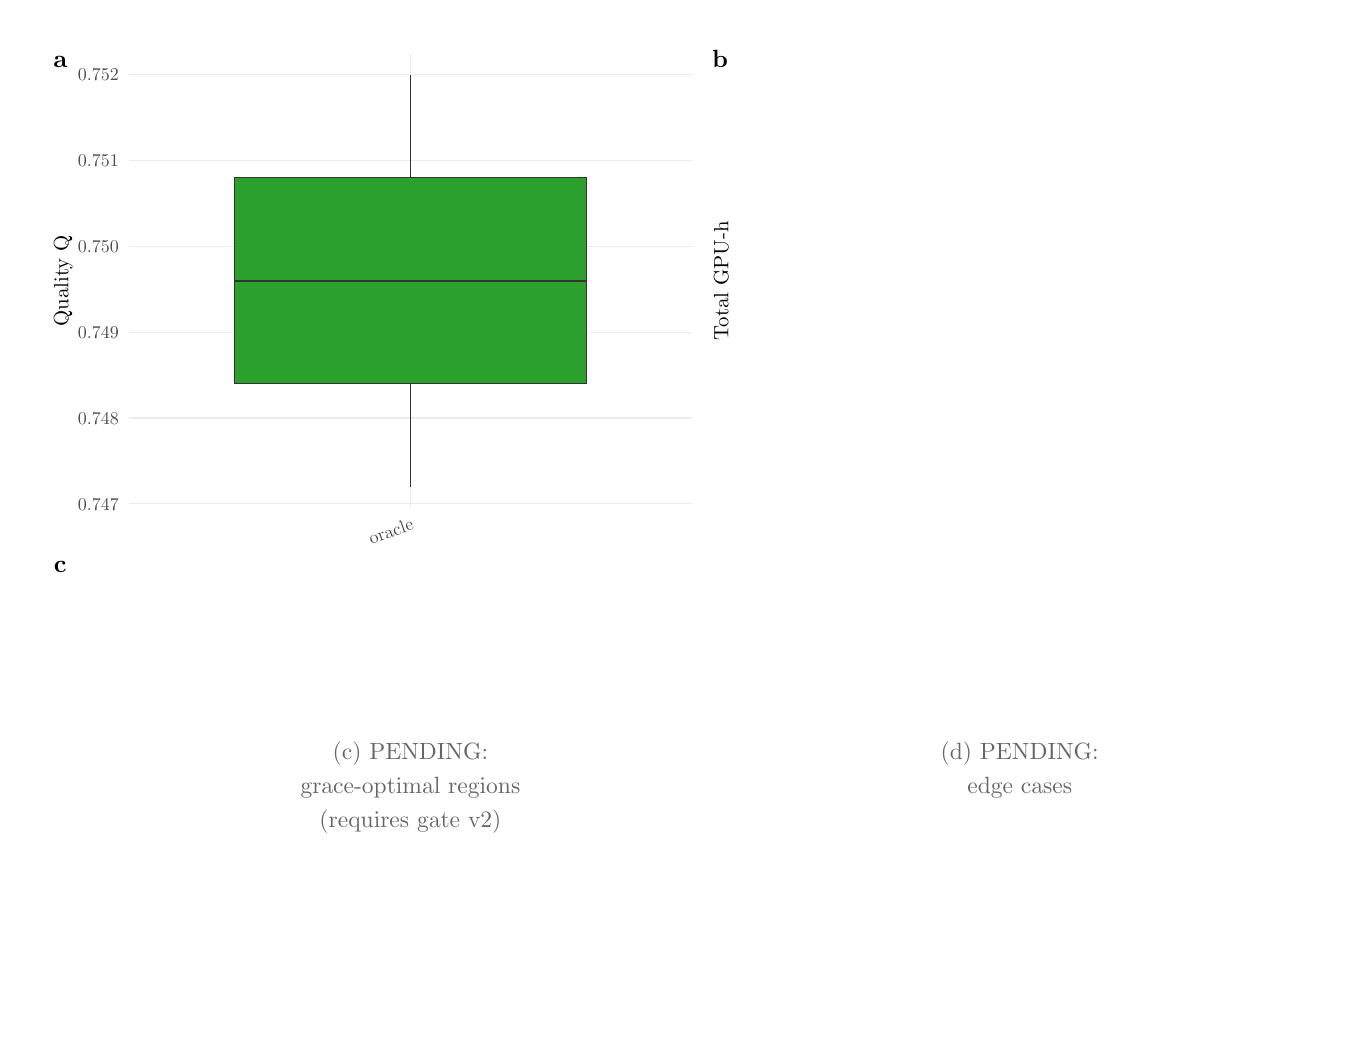
\begin{tikzpicture}[x=1pt,y=1pt]
\definecolor{fillColor}{RGB}{255,255,255}
\path[use as bounding box,fill=fillColor,fill opacity=0.00] (0,0) rectangle (469.75,361.35);
\begin{scope}
\path[clip] (  0.00,  0.00) rectangle (469.75,361.35);
\definecolor{drawColor}{RGB}{255,255,255}
\definecolor{fillColor}{RGB}{255,255,255}

\path[draw=drawColor,line width= 0.6pt,line join=round,line cap=round,fill=fillColor] (  0.00,  0.00) rectangle (469.76,361.35);
\end{scope}
\begin{scope}
\path[clip] (  5.50,169.33) rectangle (244.08,355.85);
\definecolor{fillColor}{RGB}{255,255,255}

\path[fill=fillColor] (  5.50,169.33) rectangle (244.08,355.85);
\end{scope}
\begin{scope}
\path[clip] (244.08,169.33) rectangle (464.25,355.85);
\definecolor{fillColor}{RGB}{255,255,255}

\path[fill=fillColor] (244.08,169.33) rectangle (464.25,355.85);
\end{scope}
\begin{scope}
\path[clip] (  5.50,  5.50) rectangle (244.08,169.33);

\path[] (  5.50,  5.50) rectangle (244.08,169.33);
\end{scope}
\begin{scope}
\path[clip] (244.08,  5.50) rectangle (464.25,169.33);

\path[] (244.08,  5.50) rectangle (464.25,169.33);
\end{scope}
\begin{scope}
\path[clip] ( 36.53,188.02) rectangle (240.08,351.85);
\definecolor{drawColor}{gray}{0.92}

\path[draw=drawColor,line width= 0.4pt,line join=round] ( 36.53,189.26) --
	(240.08,189.26);

\path[draw=drawColor,line width= 0.4pt,line join=round] ( 36.53,220.29) --
	(240.08,220.29);

\path[draw=drawColor,line width= 0.4pt,line join=round] ( 36.53,251.31) --
	(240.08,251.31);

\path[draw=drawColor,line width= 0.4pt,line join=round] ( 36.53,282.34) --
	(240.08,282.34);

\path[draw=drawColor,line width= 0.4pt,line join=round] ( 36.53,313.37) --
	(240.08,313.37);

\path[draw=drawColor,line width= 0.4pt,line join=round] ( 36.53,344.40) --
	(240.08,344.40);

\path[draw=drawColor,line width= 0.4pt,line join=round] (138.30,188.02) --
	(138.30,351.85);
\definecolor{drawColor}{gray}{0.20}

\path[draw=drawColor,line width= 0.4pt,line join=round] (138.30,307.17) -- (138.30,344.40);

\path[draw=drawColor,line width= 0.4pt,line join=round] (138.30,232.70) -- (138.30,195.46);
\definecolor{fillColor}{RGB}{44,160,44}

\path[draw=drawColor,line width= 0.4pt,fill=fillColor] ( 74.69,307.17) --
	( 74.69,232.70) --
	(201.91,232.70) --
	(201.91,307.17) --
	( 74.69,307.17) --
	cycle;

\path[draw=drawColor,line width= 0.8pt] ( 74.69,269.93) -- (201.91,269.93);
\end{scope}
\begin{scope}
\path[clip] (  0.00,  0.00) rectangle (469.75,361.35);
\definecolor{drawColor}{gray}{0.30}

\node[text=drawColor,anchor=base east,inner sep=0pt, outer sep=0pt, scale=  0.65] at ( 32.93,187.02) {0.747};

\node[text=drawColor,anchor=base east,inner sep=0pt, outer sep=0pt, scale=  0.65] at ( 32.93,218.05) {0.748};

\node[text=drawColor,anchor=base east,inner sep=0pt, outer sep=0pt, scale=  0.65] at ( 32.93,249.08) {0.749};

\node[text=drawColor,anchor=base east,inner sep=0pt, outer sep=0pt, scale=  0.65] at ( 32.93,280.11) {0.750};

\node[text=drawColor,anchor=base east,inner sep=0pt, outer sep=0pt, scale=  0.65] at ( 32.93,311.14) {0.751};

\node[text=drawColor,anchor=base east,inner sep=0pt, outer sep=0pt, scale=  0.65] at ( 32.93,342.16) {0.752};
\end{scope}
\begin{scope}
\path[clip] (  0.00,  0.00) rectangle (469.75,361.35);
\definecolor{drawColor}{gray}{0.30}

\node[text=drawColor,rotate= 20.00,anchor=base east,inner sep=0pt, outer sep=0pt, scale=  0.65] at (139.83,180.21) {oracle};
\end{scope}
\begin{scope}
\path[clip] (  0.00,  0.00) rectangle (469.75,361.35);
\definecolor{drawColor}{RGB}{0,0,0}

\node[text=drawColor,rotate= 90.00,anchor=base,inner sep=0pt, outer sep=0pt, scale=  0.75] at ( 14.67,269.93) {Quality Q};
\end{scope}
\begin{scope}
\path[clip] (  0.00,  0.00) rectangle (469.75,361.35);
\definecolor{drawColor}{RGB}{0,0,0}

\node[text=drawColor,anchor=base,inner sep=0pt, outer sep=0pt, scale=  0.90] at ( 11.81,346.96) {\bfseries a};
\end{scope}
\begin{scope}
\path[clip] (  0.00,  0.00) rectangle (469.75,361.35);
\definecolor{drawColor}{RGB}{0,0,0}

\node[text=drawColor,rotate= 90.00,anchor=base,inner sep=0pt, outer sep=0pt, scale=  0.75] at (253.24,269.93) {Total GPU-h};
\end{scope}
\begin{scope}
\path[clip] (  0.00,  0.00) rectangle (469.75,361.35);
\definecolor{drawColor}{RGB}{0,0,0}

\node[text=drawColor,anchor=base,inner sep=0pt, outer sep=0pt, scale=  0.90] at (250.20,346.96) {\bfseries b};
\end{scope}
\begin{scope}
\path[clip] ( 36.53,  5.50) rectangle (240.08,169.33);
\definecolor{drawColor}{gray}{0.40}

\node[text=drawColor,anchor=base,inner sep=0pt, outer sep=0pt, scale=  0.85] at (138.30, 96.77) {(c) PENDING:};

\node[text=drawColor,anchor=base,inner sep=0pt, outer sep=0pt, scale=  0.85] at (138.30, 84.48) {grace-optimal regions};

\node[text=drawColor,anchor=base,inner sep=0pt, outer sep=0pt, scale=  0.85] at (138.30, 72.19) {(requires gate v2)};
\end{scope}
\begin{scope}
\path[clip] (  0.00,  0.00) rectangle (469.75,361.35);
\definecolor{drawColor}{RGB}{0,0,0}

\node[text=drawColor,anchor=base,inner sep=0pt, outer sep=0pt, scale=  0.90] at ( 11.81,164.59) {\bfseries c};
\end{scope}
\begin{scope}
\path[clip] (256.70,  5.50) rectangle (460.26,169.33);
\definecolor{drawColor}{gray}{0.40}

\node[text=drawColor,anchor=base,inner sep=0pt, outer sep=0pt, scale=  0.85] at (358.48, 96.77) {(d) PENDING:};

\node[text=drawColor,anchor=base,inner sep=0pt, outer sep=0pt, scale=  0.85] at (358.48, 84.48) {edge cases};
\end{scope}
\end{tikzpicture}
